\begin{frame}{Fonctionnalités de la solution : GreenT}
\vspace{-10px}
	\begin{itemize}
		\item Analyser le fichier de spécifications\newline
			\footnotesize
			$\rightarrow$ Fichier complété par un testeur au sein de Continental
			\normalsize

		\item Générer automatiquement des fichiers exécutables
		\item Rapports détaillés

	\end{itemize}
	\vfill
	\begin{figure}[H]
		\centering
		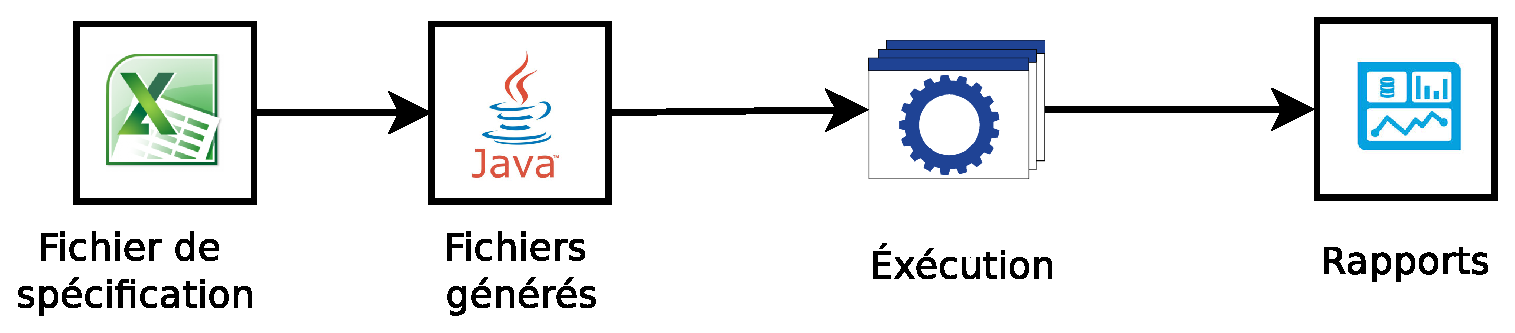
\includegraphics[width=8.5cm]{images/fct.eps}
		\caption{Fonctionnalités principales}
	\end{figure}
\end{frame}

\begin{frame}{Fonctionnement global de GreenT}
	\begin{figure}[H]
		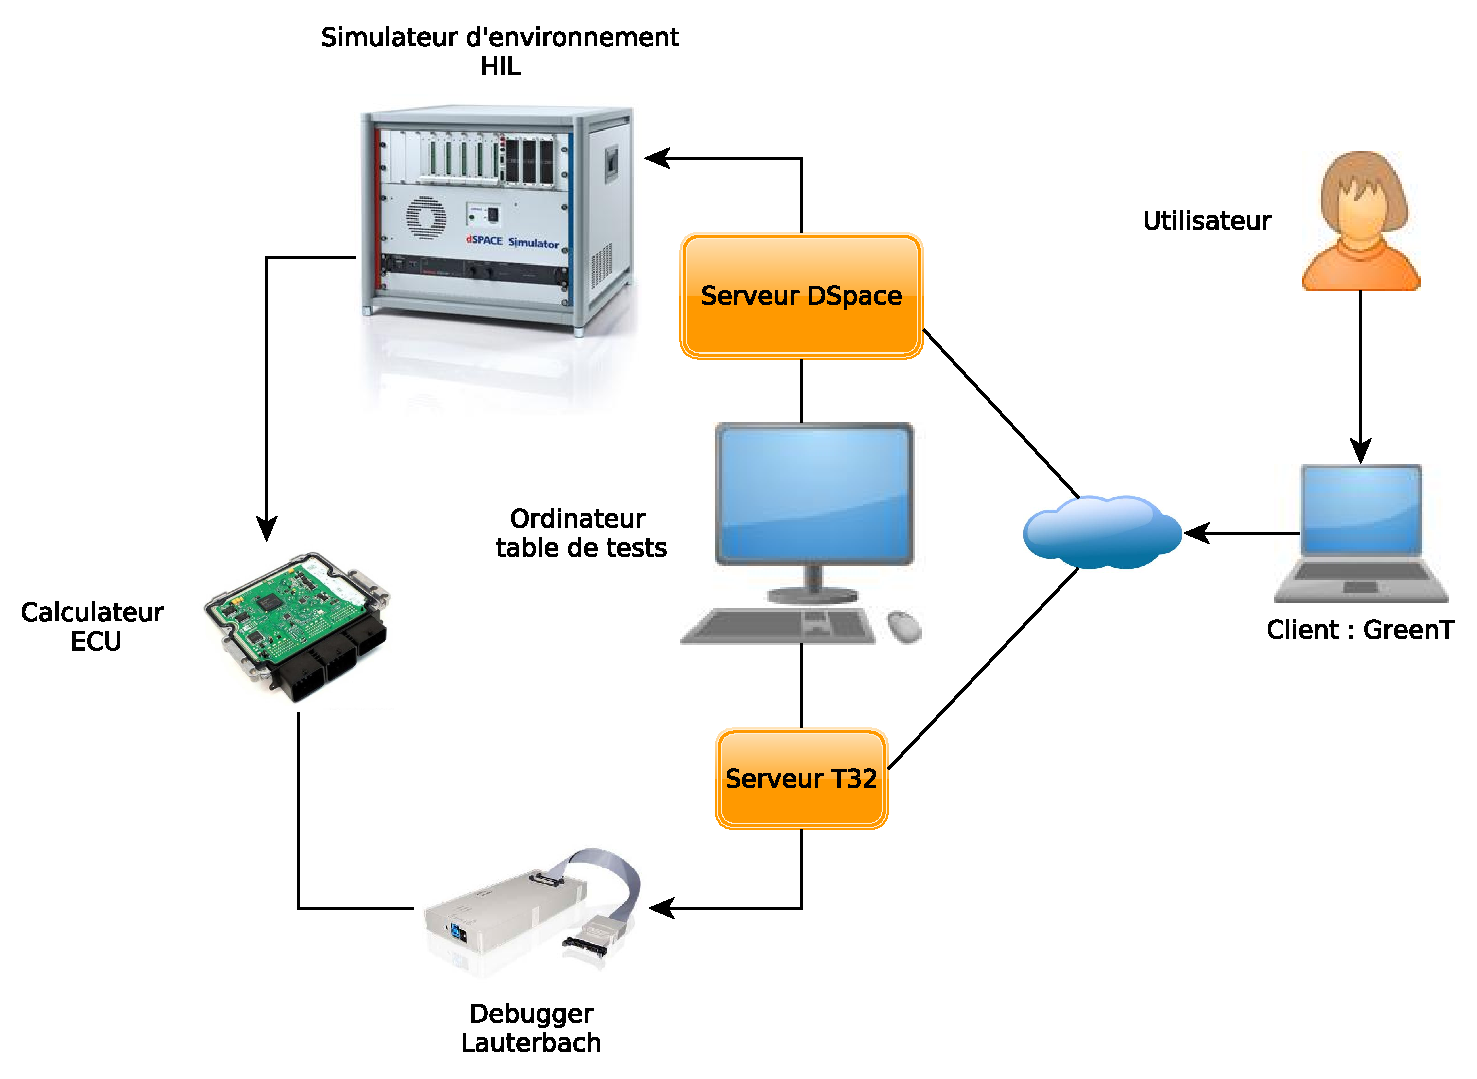
\includegraphics[width=9cm]{images/network.eps}
		\caption{Schéma de fonctionnement général}	
	\end{figure}
\end{frame}
\begin{frame}[plain]
	\begin{tikzpicture}[remember picture,overlay]
	\node[at=(current page.center)] {
		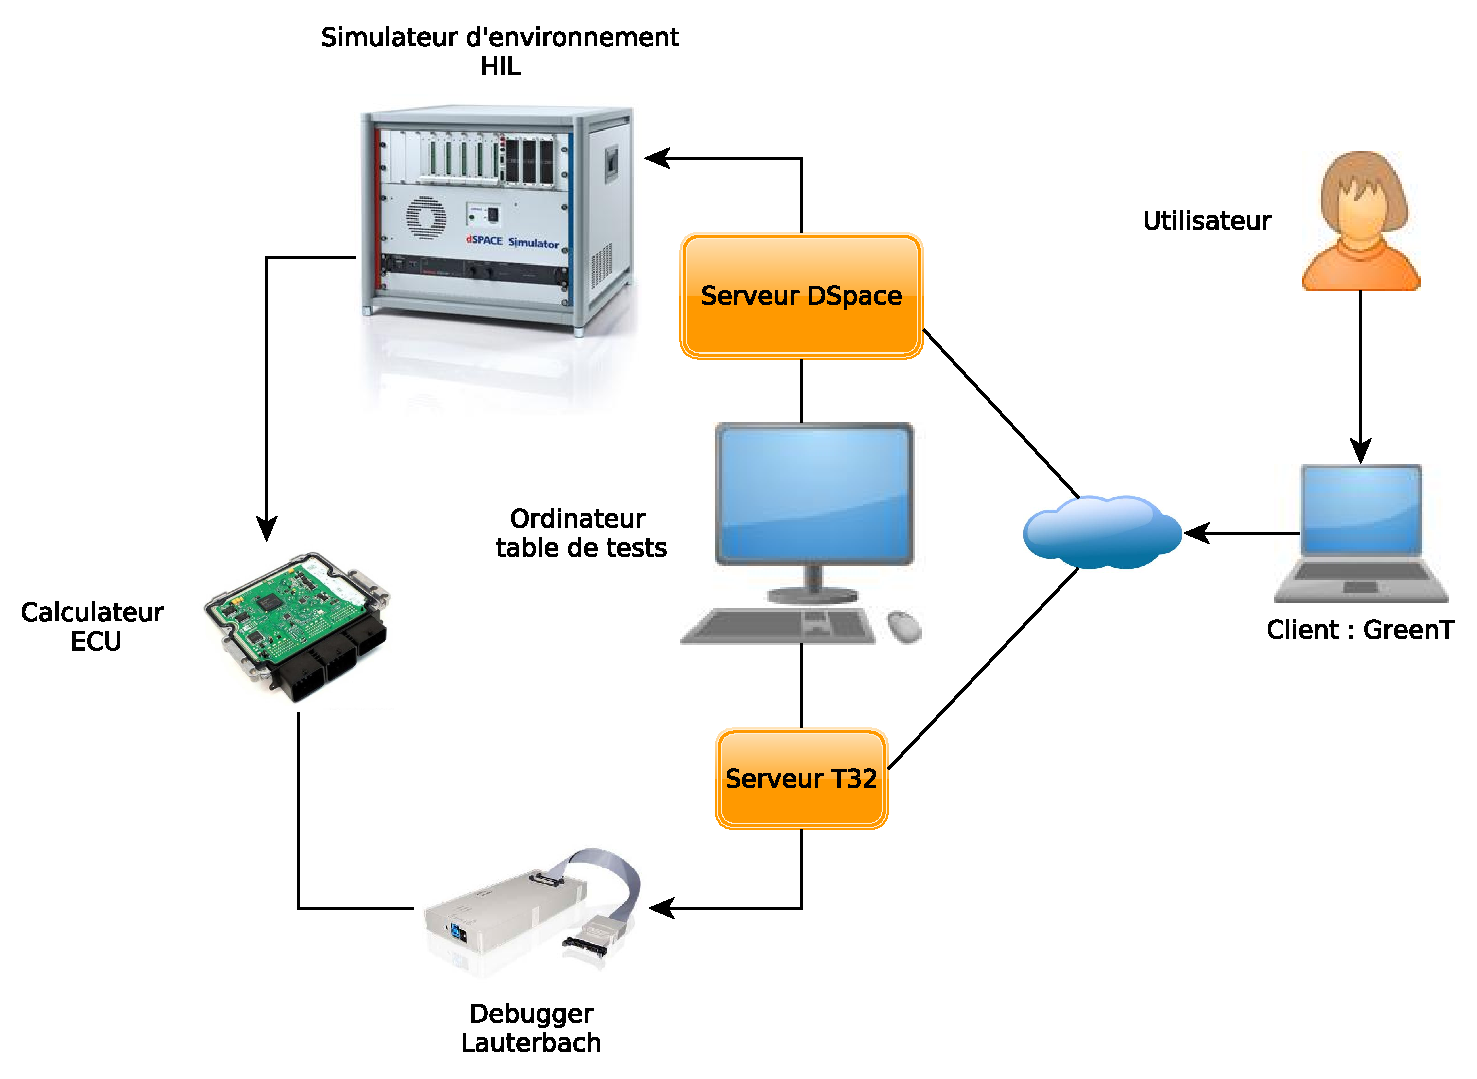
\includegraphics[width=\paperwidth]{images/network.eps}
	};
	\end{tikzpicture}
\end{frame}

\begin{frame}{Fonctionnement d'un cas de tests}
		  \setbeamercovered{transparent}
	\begin{itemize}[<+->]
	  \vfill
		\item Un scénario de précondition
		\begin{itemize}
			\item Initialise le banc de tests
		\end{itemize}
	\vfill
		\item Des scénarios de stimulation de l'environnement
			\begin{itemize}
			\item Pilotent le banc HIL 
			\item Enregistrement de variables durant les scénarios
			\end{itemize}
	\vfill
		\item \textit{Expected Behavior }
			\begin{itemize}
				\item Expression logique 
				\item Évaluée sur l'ensemble de l'enregistrement
			\end{itemize}
			\vspace{-30px}
	\end{itemize}
	\begin{figure}[H]
		\centering
		\only<1,2> {
			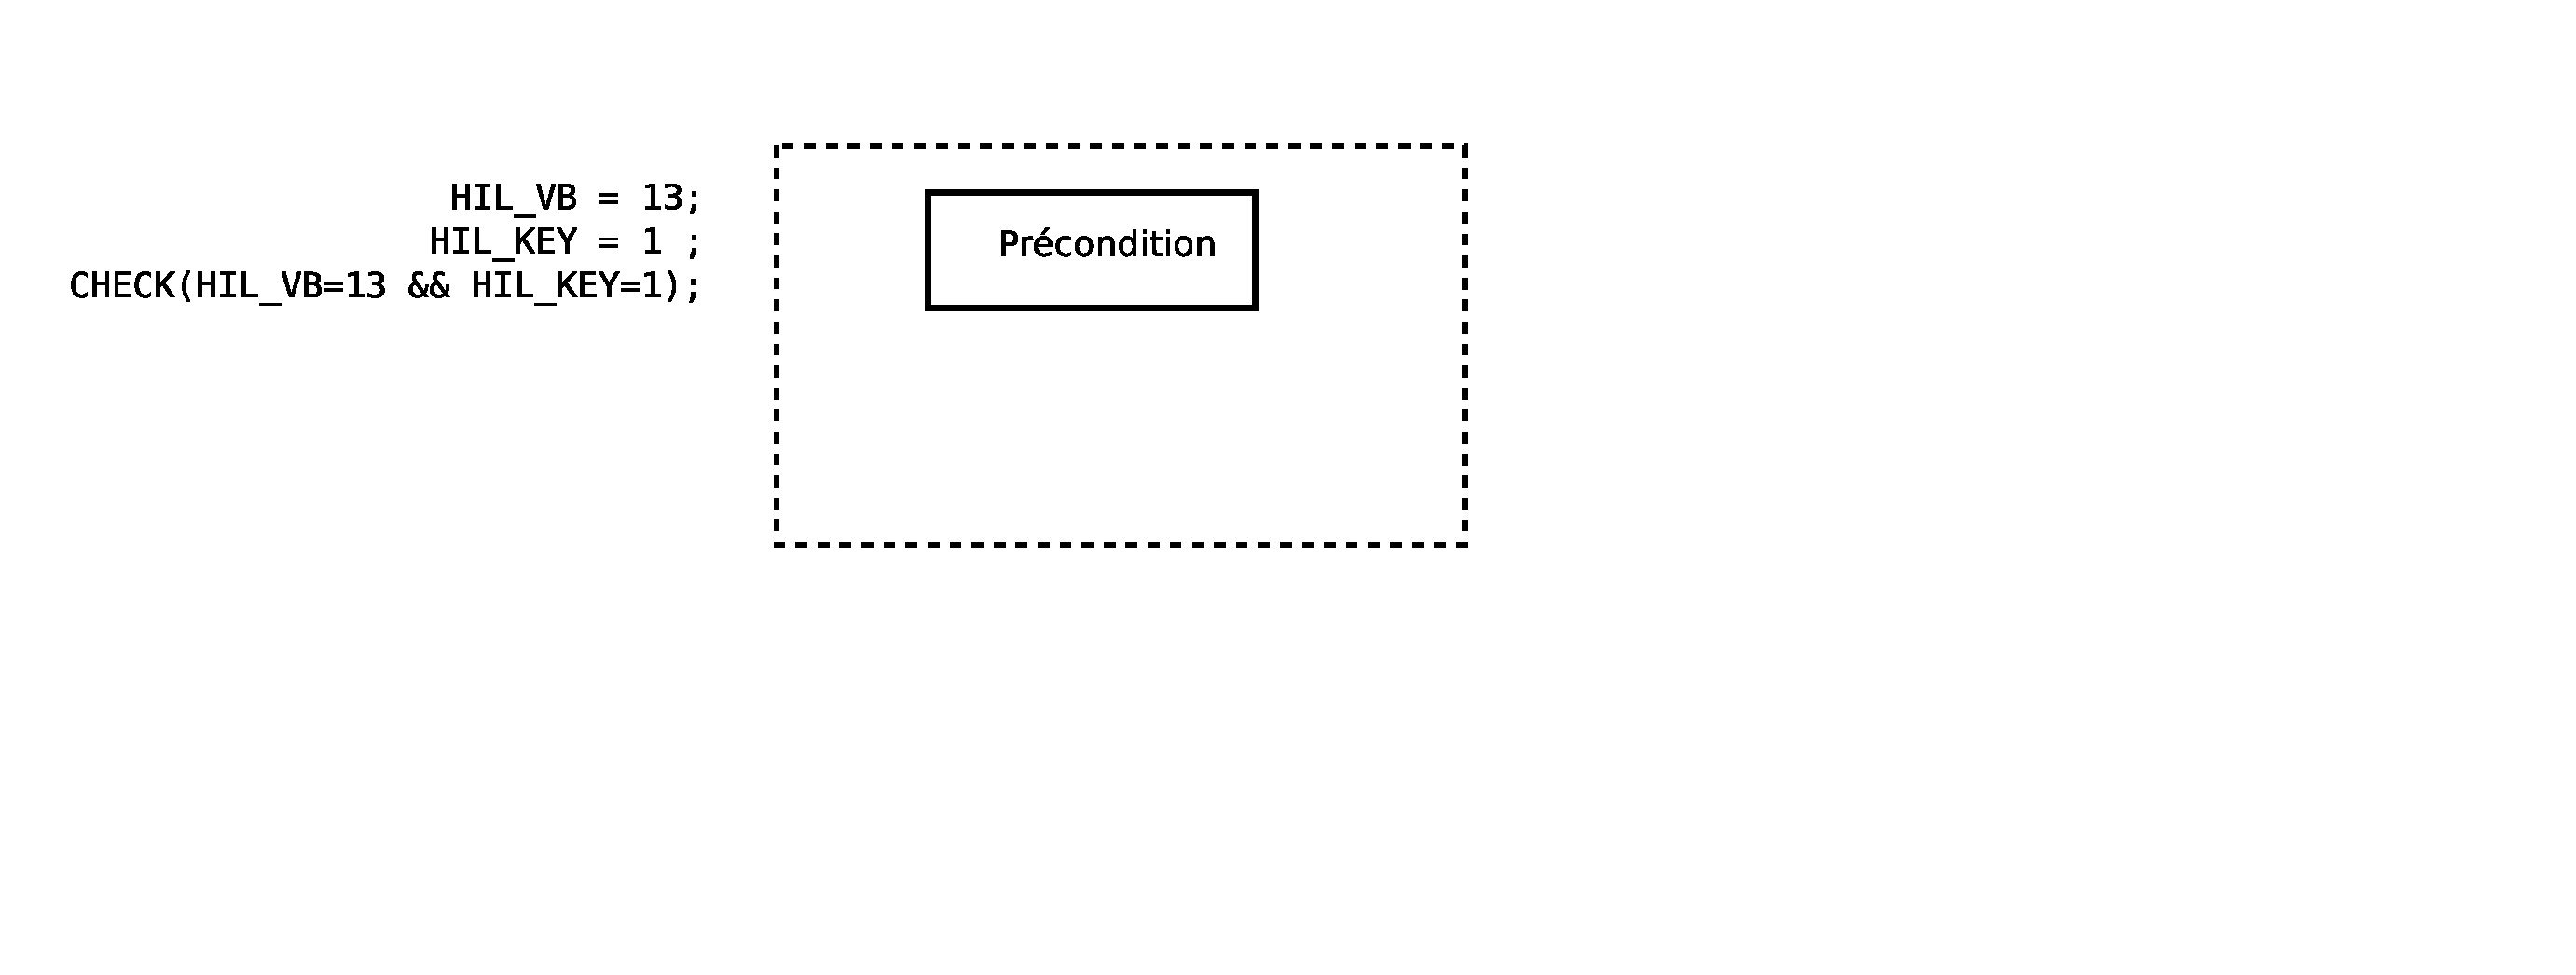
\includegraphics[width=9.5cm]{images/exe1.eps}
		}
		\only<3,4> {
			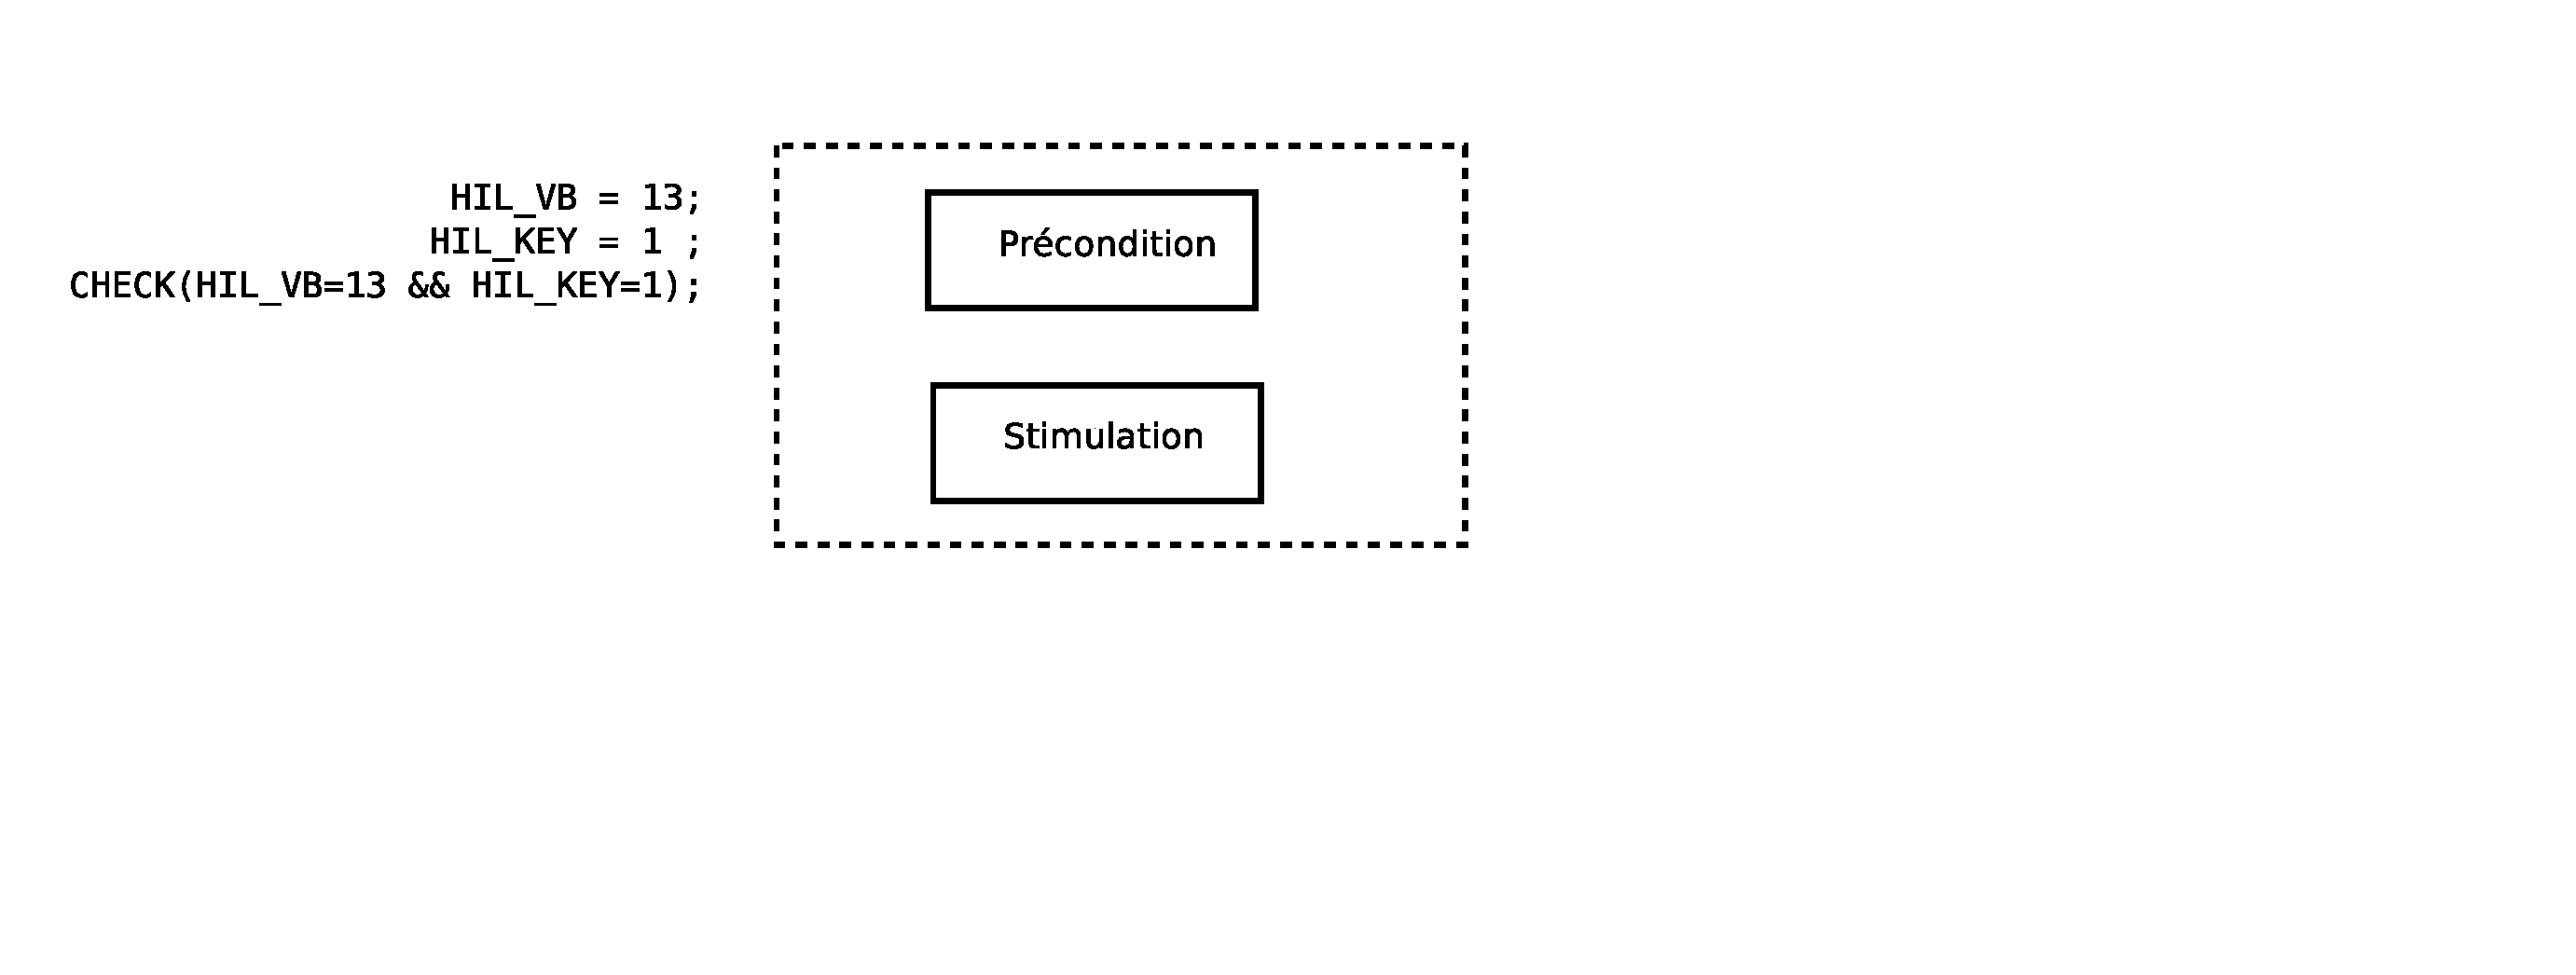
\includegraphics[width=9.5cm]{images/exe2.eps}
		}
		\only<5> {
			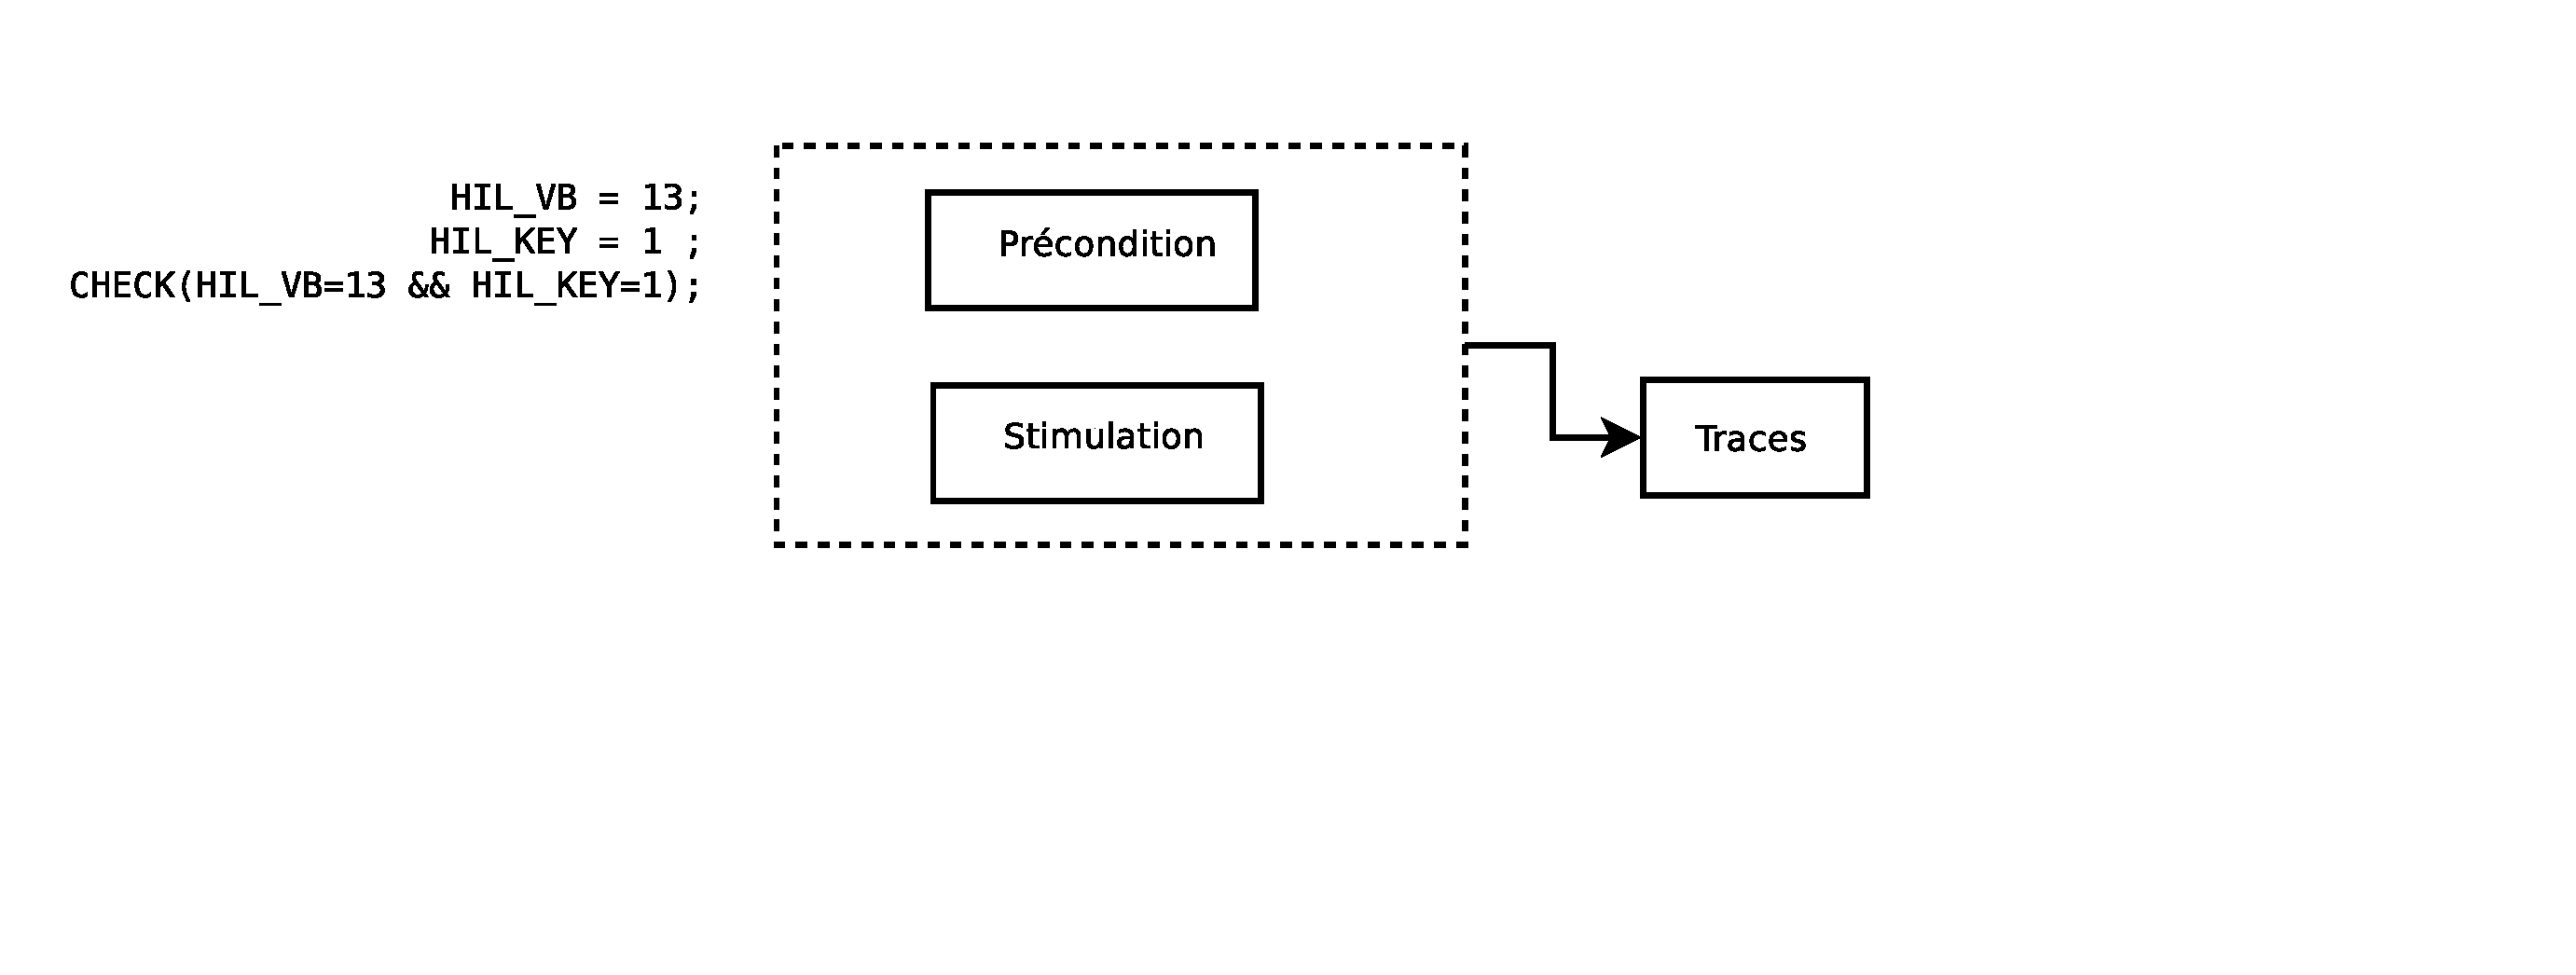
\includegraphics[width=9.5cm]{images/exe3.eps}
		}
		\only<6,7> {
			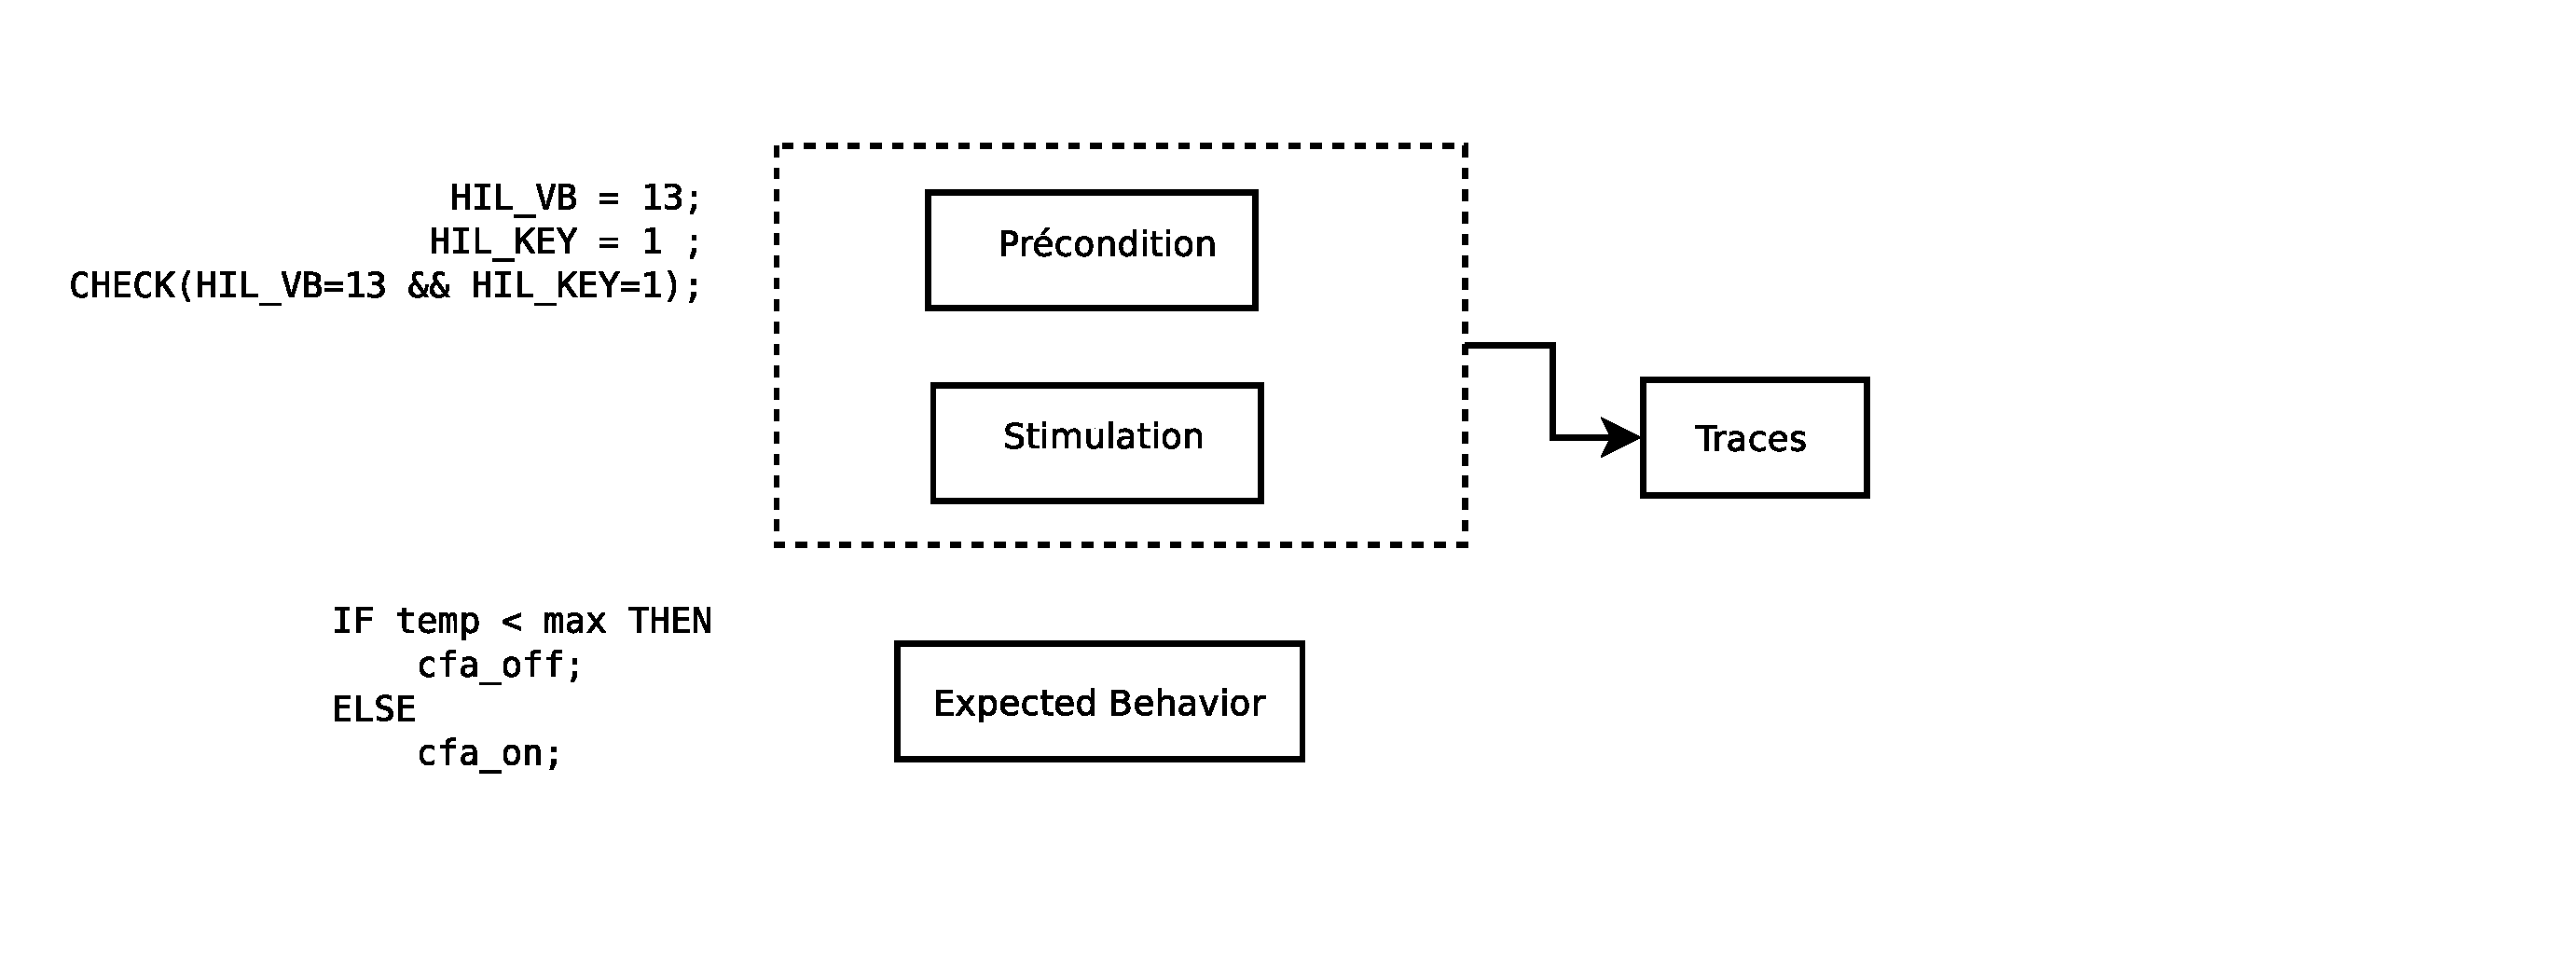
\includegraphics[width=9.5cm]{images/exe4.eps}
		}
		\only<8> {
			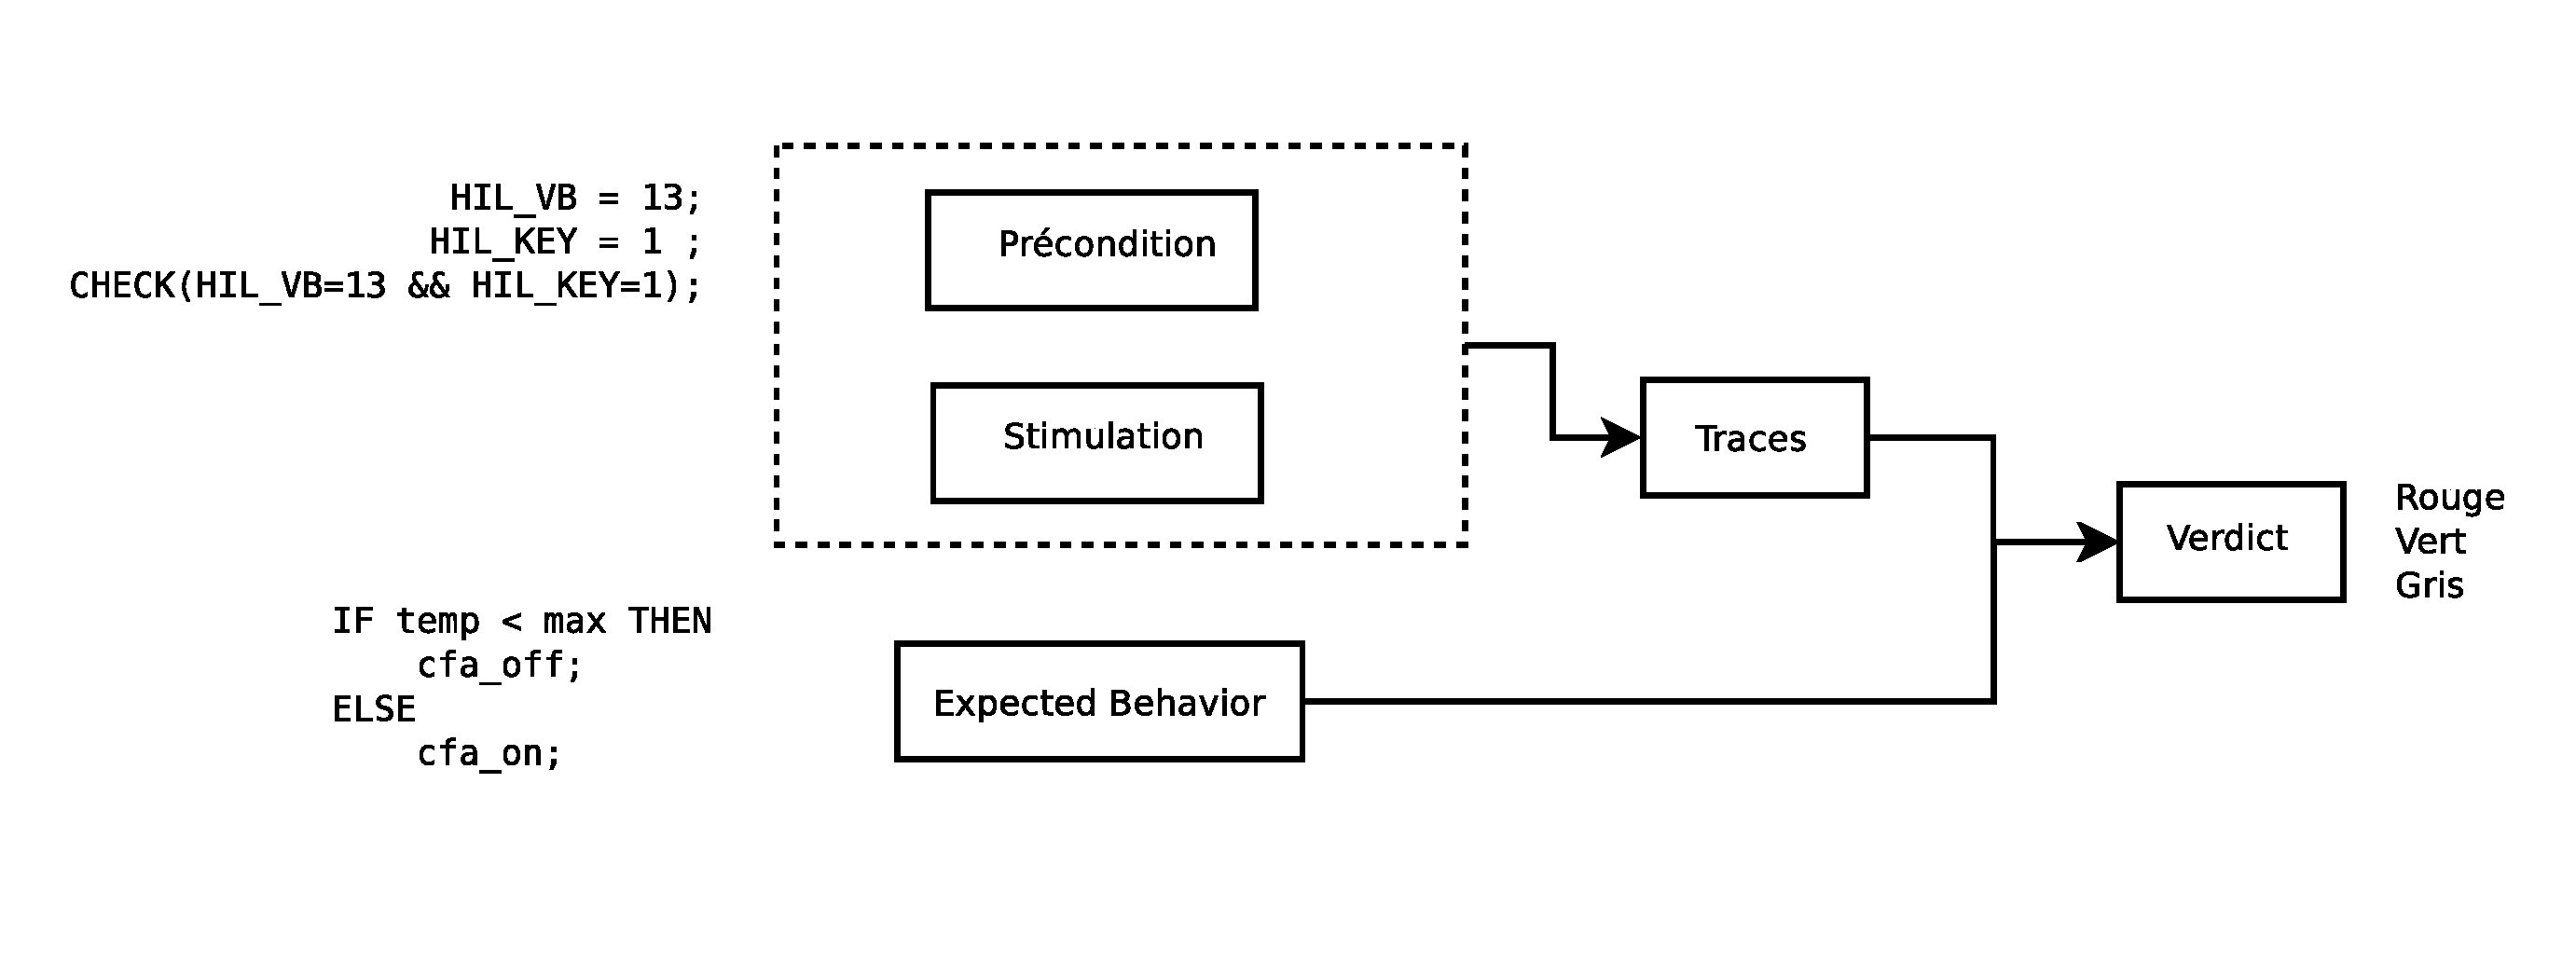
\includegraphics[width=9.5cm]{images/exe.eps}
		}
		\caption{Fonctionnement d'un exécutable}
	\end{figure}
\end{frame}



